\section{Desarrollo} \label{sect:desarrollo}

Durante esta fase se implementó progresivamente la versión alfa del prototipo funcional. 

Se creó un componente móvil y un servidor para dar solución al problema de registro y control de gastos.

Para cumplir con los requerimientos del componente móvil, se creó una aplicación para el sistema operativo Android, y se trabajó con el IDE Android Studio. 

El desarrollo de la aplicación implicó la creación de múltiples vistas (tanto interfaces de usuario como la lógica para manejar acciones de usuario), y de diversas consultas a la base de datos, muchas de las cuales realizaban modificaciones a la misma.

En primer lugar, se creó la interfaz de la vista principal de la aplicación, donde se muestra el total de ingresos, el total de gastos y el balance general (ver figura 5.6).

\begin{figure}[ht]
\centering
\begin{minipage}{.5\textwidth}
  \centering
  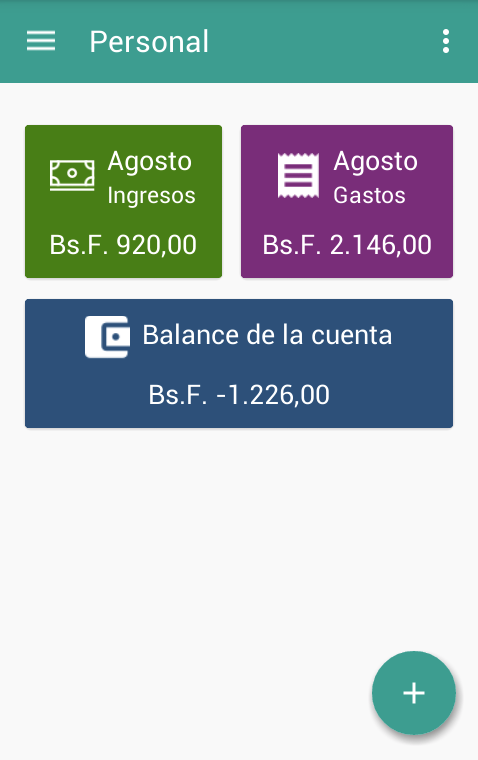
\includegraphics[scale=0.45,type=png,ext=.png,read=.png]{imagenes/dashboard}
  \captionsetup{justification=centering}
  \captionof{figure}{Interfaz principal de la\\ aplicación}
  \label{fig:interfazDashboard}
\end{minipage}%
\begin{minipage}{.5\textwidth}
\centering
  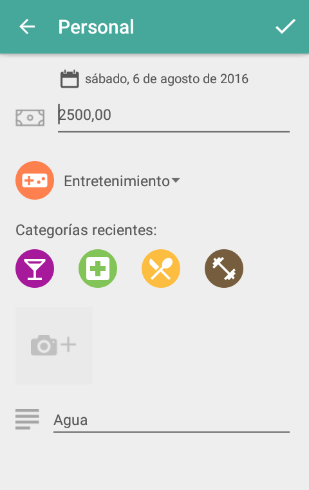
\includegraphics[scale=0.45,type=png,ext=.png,read=.png]{imagenes/create_entry}
  \captionsetup{justification=centering}
  \captionof{figure}{Interfaz para crear o editar gastos o ingresos}
  \label{fig:interfazCrearEntry}
\end{minipage}
\end{figure}

Se implementó una vista para crear y editar gastos (ver figura 5.7). Para estos gastos, se debe guardar su monto, fecha, descripción, fotos de recibos y categoría a la que pertenecen. Posteriormente, se decidió extender la funcionalidad de creación de gastos para permitir también el manejo de ingresos. 

Para mostrar los gastos e ingresos guardados, se creó una vista para listarlos (ver figuras 5.8 y 5.9). En las listas se muestran la descripción/categoría a la que pertenece cada entrada, su monto y su fecha. Dentro de cada lista, se permite ver los detalles de cada gasto/ingreso, editarlos y eliminarlos. Además, también se permite filtrar las listas por palabras claves.

\begin{figure}[ht]
\centering
\begin{minipage}{.5\textwidth}
  \centering
  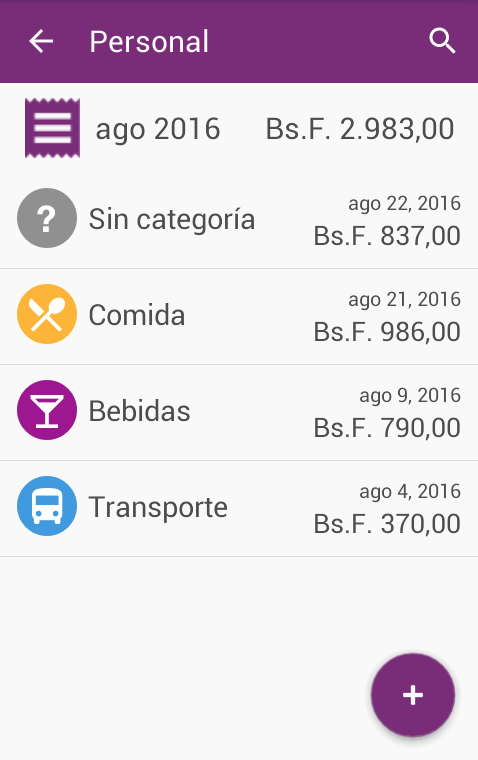
\includegraphics[scale=0.45,type=png,ext=.png,read=.png]{imagenes/expenses_list}
  \captionsetup{justification=centering}
  \captionof{figure}{Interfaz para listar gastos}
  \label{fig:interfazListarExpenses}
\end{minipage}%
\begin{minipage}{.5\textwidth}
\centering
  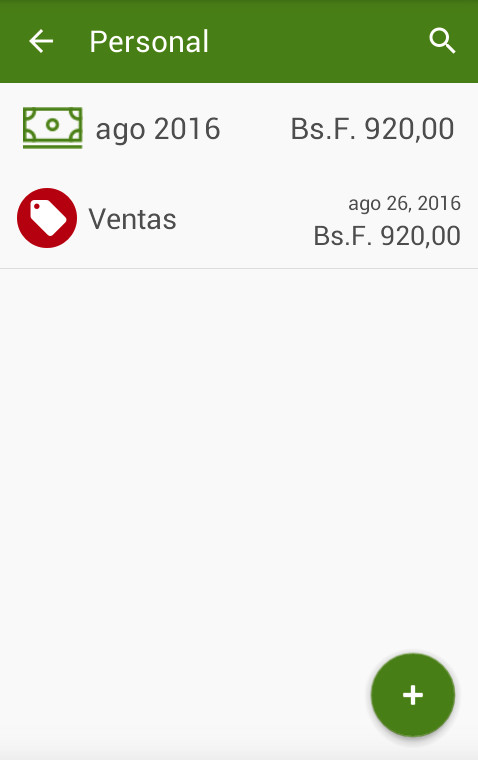
\includegraphics[scale=0.45,type=png,ext=.png,read=.png]{imagenes/incomes_list}
  \captionsetup{justification=centering}
  \captionof{figure}{Interfaz para listar ingresos}
  \label{fig:interfazListarIncomes}
\end{minipage}
\end{figure}

También se crearon vistas para el manejo de categorías. Se creó una vista para la creación/edición de categorías, y otra para listarlas (ver figuras 5.10 y 5.11). Estas categorías pueden ser de dos tipos: categorías de gastos o categorías de ingresos.

\begin{figure}[ht]
\centering
\begin{minipage}{.5\textwidth}
  \centering
  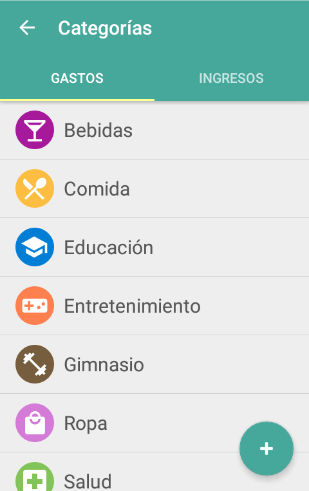
\includegraphics[scale=0.45,type=png,ext=.png,read=.png]{imagenes/expense_categories}
  \captionsetup{justification=centering}
  \captionof{figure}{Interfaz para listar categorías\\ de gastos}
  \label{fig:interfazListarExpensesCategories}
\end{minipage}%
\begin{minipage}{.5\textwidth}
\centering
  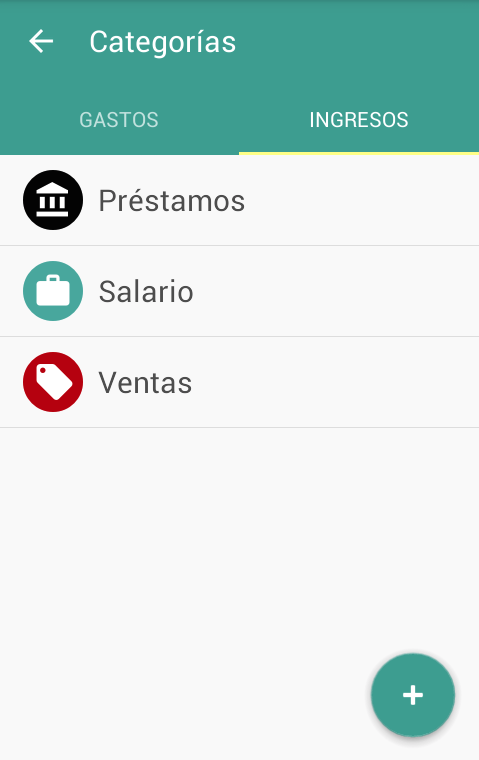
\includegraphics[scale=0.45,type=png,ext=.png,read=.png]{imagenes/income_categories}
  \captionsetup{justification=centering}
  \captionof{figure}{Interfaz para listar categorías\\ de ingresos}
  \label{fig:interfazListarIncomesCategories}
\end{minipage}
\end{figure}

Luego de la creación de las principales funcionalidades del sistema, mencionadas en los párrafos anteriores, se introdujo el concepto de \textit{cuentas}. Hasta el momento, los gastos estaban asociados a una única cuenta por defecto. Por esta razón, también se creó una funcionalidad para agregar nuevas cuentas, y poder crear nuevos gastos dentro de dichas cuentas. Estas cuentas pueden ser de dos tipos: activas o archivadas; la navegación entre cuentas se hace únicamente con las cuentas activas. 

Además, también se creó una vista para poder listar las cuentas creadas y guardadas en el dispositivo (ver figuras 5.12 y 5.13). A partir de esta vista, se puede editar, eliminar o cambiar el estado de las cuentas (activa o archivada).


\begin{figure}[ht]
\centering
\begin{minipage}{.5\textwidth}
  \centering
  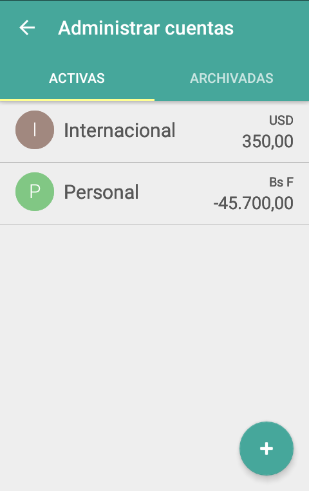
\includegraphics[scale=0.45,type=png,ext=.png,read=.png]{imagenes/active_accounts}
  \captionsetup{justification=centering}
  \captionof{figure}{Interfaz para listar cuentas\\ activas}
  \label{fig:interfazListarActiveAccounts}
\end{minipage}%
\begin{minipage}{.5\textwidth}
\centering
  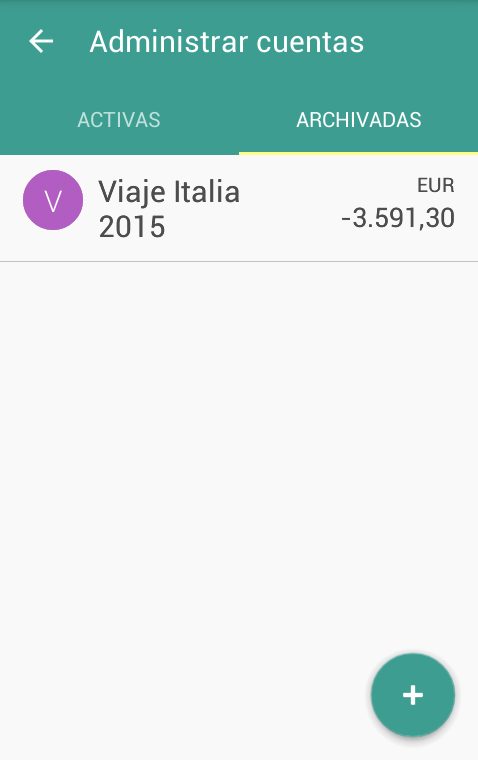
\includegraphics[scale=0.45,type=png,ext=.png,read=.png]{imagenes/archived_accounts}
  \captionsetup{justification=centering}
  \captionof{figure}{Interfaz para listar cuentas archivadas}
  \label{fig:interfazListarArchivedAccounts}
\end{minipage}
\end{figure}

Como se explicó en la sección anterior, es necesario guardar toda esta información en la base de datos local de cada dispositivo. Para ello, se utilizó la librería SQLite.

Además, también se crearon dos vistas para reportes de gastos: una para reportes de balance general, y otra para reporte de gastos por categorías (ver figuras 5.14 y 5.15).

La vista de reporte de balance general muestra una lista de gastos e ingresos filtrados por fecha. La vista de reporte por categorías muestra una lista de categorías con la suma total de los gastos e ingresos de dichas categorías, filtradas por fecha.

\begin{figure}[ht]
\centering
\begin{minipage}{.5\textwidth}
  \centering
  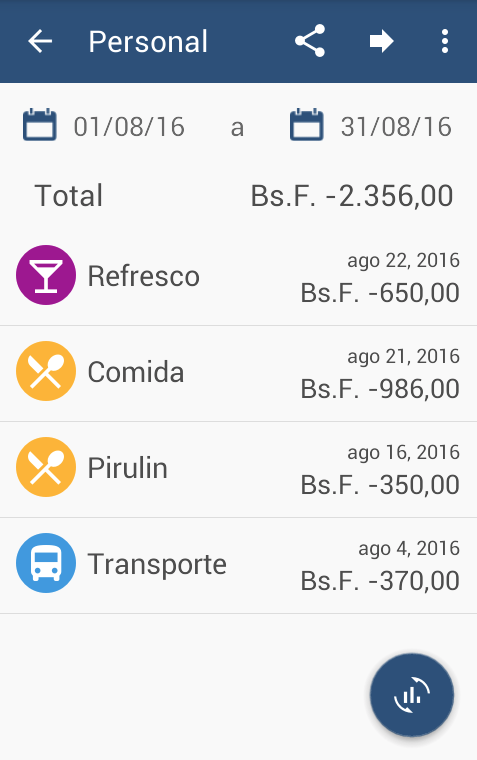
\includegraphics[scale=0.45,type=png,ext=.png,read=.png]{imagenes/balance_report}
  \captionsetup{justification=centering}
  \captionof{figure}{Interfaz para mostrar reporte\\ de balance general}
  \label{fig:interfazBalanceReport}
\end{minipage}%
\begin{minipage}{.5\textwidth}
\centering
  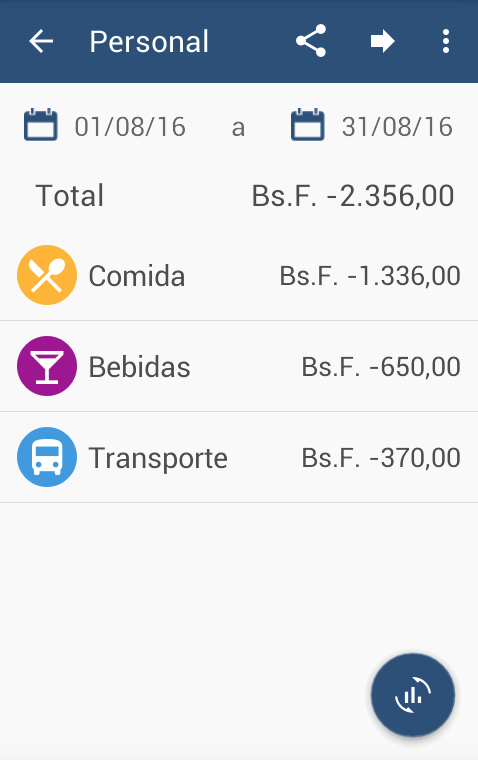
\includegraphics[scale=0.45,type=png,ext=.png,read=.png]{imagenes/categories_report}
  \captionsetup{justification=centering}
  \captionof{figure}{Interfaz para mostrar reporte\\ por categorías}
  \label{fig:interfazCategoriesReport}
\end{minipage}
\end{figure}

Para mantener la lógica separada de la interfaz gráfica, se utilizó el patrón de arquitectura MVP o Modelo Vista Presentador, descrito en el capítulo 2. De esta manera, toda acción en la vista que requiera realizar operaciones sobre la base de datos, se realizó por medio de una capa intermedia: el presentador. 

Para lograr esto, fue necesario en primer lugar implementar el modelo descrito en la figura 5.4. Se creó la base de datos con cada una de sus tablas, así como las clases (POJO's) que permitieron dar un nivel de abstracción mayor para el mapeo con la base de datos.

También se crearon las vistas necesarias, lo que incluyó tanto las interfaces gráficas como la lógica necesaria para manejar las acciones del usuario (actividades). Para cada vista, se creó una clase que actuó como la capa de presentador, quien era invocado por la vista para realizar acciones sobre el modelo. La vista se encargó de la creación de los objetos correspondientes al modelo, para luego pedir alguna acción al presentador sobre dichos objetos. El presentador tenía la función de invocar al modelo para realizar los cambios necesarios en la base de datos.

Por otra parte, se creó un servidor al que se pueda enviar información desde la aplicación móvil. 

Para permitir el acceso a la aplicación móvil, se creó un servicio web que permita hacer la autenticación del usuario. La aplicación envía al servidor un JSON con los datos del usuario (nombre de usuario y contraseña) por medio de una petición HTTP POST.

Se creó un servicio web que recibe un archivo PDF que contiene el reporte de gastos. Además del archivo, recibe la suma de gastos por cada categoría y el total de gastos. Estos datos se enviaron por medio de una petición HTTP Post Multipart, compuesta por un archivo y un JSON. Para la conversión de objetos de Java a JSON, y viceversa, se utilizó la librería GSON tanto en el servidor como en la aplicación móvil. Para persistir esta información, se utilizó Hibernate y MySQL como manejador de base de datos.

También se creó una aplicación web que permita aprobar o rechazar los reportes enviados al servidor, así como ver los reportes recibidos y ya revisados (ver figuras 5.16 y 5.17). Además de esto, la herramienta utilizada para el desarrollo del servidor trae consigo algunas funcionalidades por defecto: iniciar sesión y el manejo de usuarios (agregar, modificar y eliminar usuarios).

\begin{figure}[ht]
  \centering
  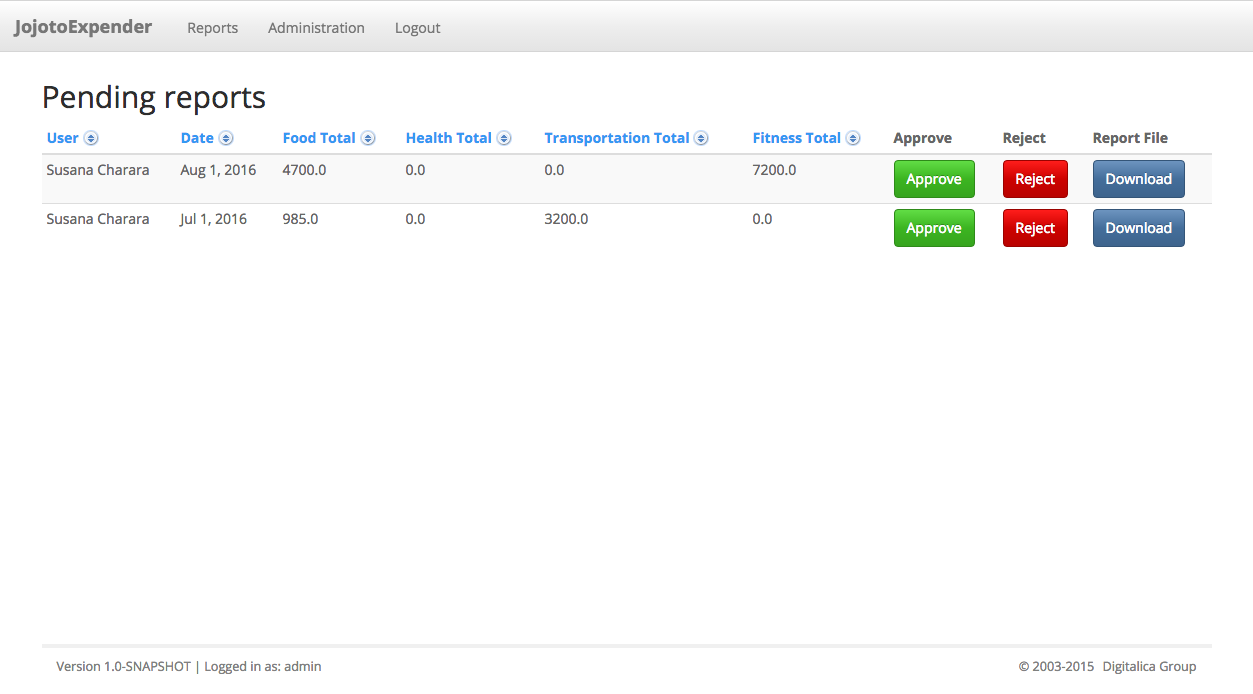
\includegraphics[scale=0.35,type=png,ext=.png,read=.png]{imagenes/pending_reports}
  \captionsetup{justification=centering}
  \caption{Interfaz para listar reportes pendientes de revisión}
  \label{fig:interfazListarReportesPendientes}
\end{figure}

\begin{figure}[h]
  \centering
  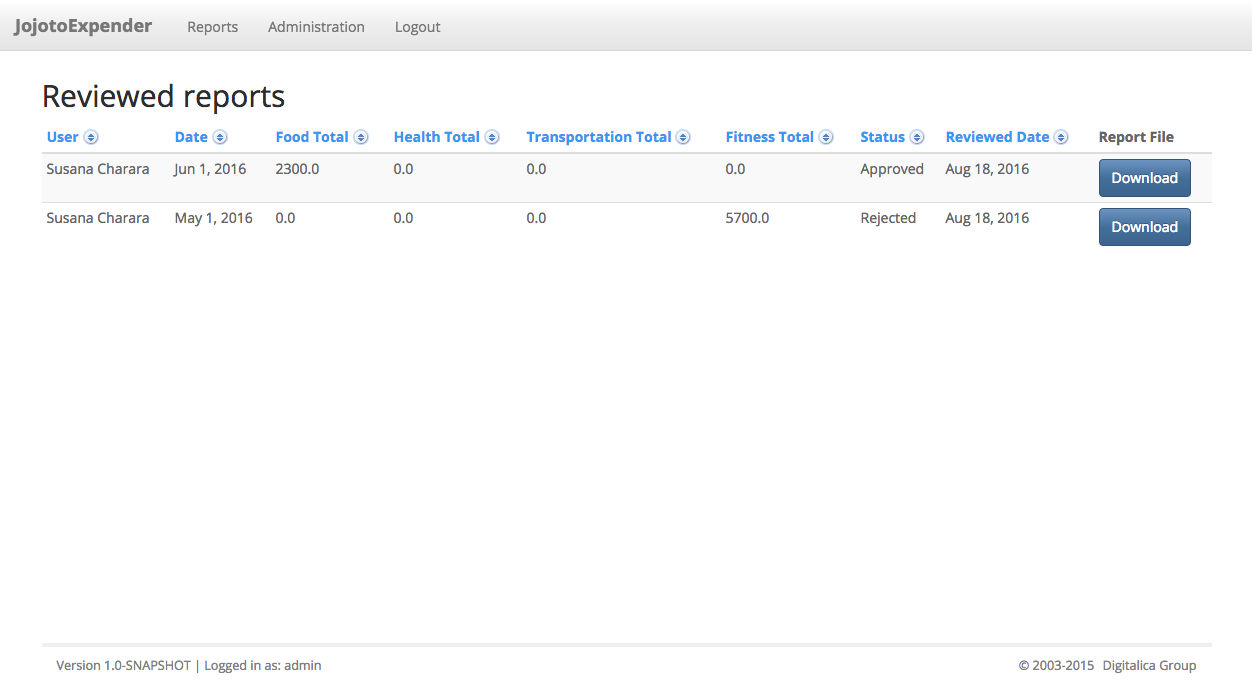
\includegraphics[scale=0.35,type=png,ext=.png,read=.png]{imagenes/reviewed_reports}
  \captionsetup{justification=centering}
  \caption{Interfaz para listar reportes aprobados/rechazados}
  \label{fig:interfazListarReportesRevisados}
\end{figure}

El desarrollo del componente servidor se realizó con el IDE Eclipse. Se utilizó el \textit{framework} AppFuse, que integra a su vez otros \textit{frameworks} que facilitan el desarrollo web. En este caso, se trabajó en conjunto con Spring y Tapestry.

Se utilizó Spring para la implementación de los servicios web que permiten recibir datos desde la aplicación móvil. Estos servicios se implementaron utilizando el patrón \textit{Facade}, mediante una clase \textit{Manager}, la cual accede a los POJO's mediante un DAO (para más información, ver capítulo 2). Además, Spring también cuenta con el \textit{framework} Hibernate para la persistencia de los datos, utilizando como manejador de base de datos MySQL.

Para crear la aplicación web, se utilizó Tapestry. Con Jetty se proveen los servicios, mediante el protocolo HTTP, que permiten la comunicación con la aplicación web y la aplicación  móvil.

Por otra parte, a través de la librería Retrofit, la aplicación se comunica con el servidor web utlizando el protocolo HTTP. La comunicación con la base de datos del dispositivo y con los servicios web se realizan en la capa del presentador. Por su parte, en la vista se maneja toda la interfaz gráfica a través de la cual el usuario interactúa con la aplicación, y toda la lógica necesaria para la comunicación con la capa de modelo y el presentador.

El proyecto se desarrolló bajo el marco de trabajo de \textit{Scrum}, descrito en el capítulo 1. Durante la ejecución de las iteraciones, se implementaron las funcionalidades planificadas, así como las pruebas necesarias para validarlas.

A continuación se presentarán las iteraciones (\textit{sprints}), durante las cuales se desarrollaron las funcionalidades descritas en los párrafos anteriores. Para cada iteración, se mencionarán sus objetivos, resultados y una breve descripción de las actividades realizadas.

\subsection{Iteración 1}

\subsubsection{Objetivos}
	\begin{itemize}
	\item Mostrar información del balance de una cuenta
	\item Permitir la creación de un nuevo gasto
	\end{itemize}

\subsubsection{Resultados}
\begin{itemize}
\item Se creó una vista para mostrar el total de ingresos, gastos y balance general de una cuenta.
\item Se creó una vista para permitir la creación de un nuevo gasto.
\end{itemize}

\subsubsection{Actividades}
En la primera parte de la iteración se implementó el modelo de datos del dispositivo móvil, lo que implicó la creación de la base de datos con sus tablas, así como los POJO's correspondientes.

Se creó la vista principal de la aplicación móvil, donde se muestra el total de ingresos y el de gastos, así como el balance general. Para esto, fue necesario crear consultas a la base de datos que permitieran obtener el total de ingresos/gastos de una cuenta.  También se realizó una consulta que permite obtener el balance total de una cuenta.

Por otro lado se implementó una vista que permite crear un nuevo gasto, con su fecha, monto y descripción.

%Como se expuso anteriormente, la comunicación entre el modelo y la vista se hace a través de una capa intermedia: el presentador. Por esta razón, también fue necesaria la creación de un presentador para cada vista que permita hacer consultas a la base de datos.

\subsection{Iteración 2}

\subsubsection{Objetivos}
\begin{itemize}
\item Mostrar la lista de categorías
\item Permitir la creación de un nuevo ingreso
\item Permitir guardar fotos de un ingreso/gasto
\item Asociar un ingreso/gasto a una categoría
\end{itemize}

\subsubsection{Resultados}
\begin{itemize}
\item Se creó una vista para mostrar la lista de categorías a las que puede pertenecer un gasto.
\item Se adaptó y reutilizó la vista existente para crear un gasto para permitir la creación de un ingreso
\item Se agregó la funcionalidad para tomar fotos relacionadas a un ingreso/gasto
\item Se agregó la funcionalidad para poder asociar un ingreso/gasto a una categoría existente

\end{itemize}

\subsubsection{Actividades}

En esta iteración se creó la vista para mostrar las categorías presentes en el dispositivo.

Se creó una consulta para guardar en la base de datos una nueva categoría con su nombre y un ícono que la represente. Además, se creó una consulta para guardar en la base de datos una lista de categorías por defecto.

También se adaptó la vista existente para la creación de un gasto, de manera que se pueda reutilizar esta vista para la creación de un ingreso. 

Por otra parte, se implementó la funcionalidad para tomar y guardar fotos asociadas a un ingreso/gasto. Para esto se tuvo que crear un método que permita abrir la aplicación de la cámara del dispositivo desde la aplicación móvil. Luego, se tuvo que adaptar la vista para la creación de un ingreso/gasto para mostrar las miniaturas de las fotos tomadas. Se puso un límite por parte de la empresa para que el máximo de fotos que se puedan guardar por ingreso/gasto sean 3.

Por último, se modificó la vista para la creación de un ingreso/gasto para que se permitiera asociar una categoría. Se tenía como requerimiento guardar las cuatro categorías que se utilizaron más recientemente. Para esto, se tuvo que crear los métodos necesarios para persistir en el dispositivo móvil las categorías más recientes. Dado que esta información no tiene una estructura compleja, se decidió utilizar un objeto que provee la plataforma de Android, llamado \textit{SharedPreferences}, que permite guardar un conjunto de pares clave-valor. En este caso, se guardó una lista con las categorías más recientes.

\subsection{Iteración 3}
\subsubsection{Objetivos}
\begin{itemize}
\item Mostrar la lista de ingresos/gastos del mes actual
\item Mostrar los detalles de los ingresos/gastos existentes
\item Permitir editar y borrar un ingreso/gasto existente
\item Implementar una calculadora para guardar el monto de un ingreso/gasto
\end{itemize}

\subsubsection{Resultados}
\begin{itemize}
\item Se creó la vista para mostrar una lista con los gastos y otra con los ingresos del mes actual.
\item Se agregó la funcionalidad para ver los detalles de un ingreso/gasto ya existente, y poder editarlo
\item Se agregó la funcionalidad para eliminar ingresos/gastos
\item Se creó la interfaz para usar la calculadora que permita ingresar el monto de un ingreso/gasto
\end{itemize}

\subsubsection{Actividades}
En primer lugar, se adaptó la vista principal de la aplicación para mostrar el total de ingresos y gastos únicamente durante el mes actual. Para esto, se tuvo que modificar la consulta a la base de datos para obtener el total de ingresos/gastos dado un rango de fecha.

Se implementó la funcionalidad para navegar a la lista de ingresos o de gastos del mes desde la vista principal de la aplicación. Para esto, se creó una vista general donde se pueda mostrar una lista de ingresos/gastos, con su descripción (o categoría, en caso de que no tenga descripción), su fecha y su monto.

Por otra parte, se creó la funcionalidad para eliminar ingresos/gastos existentes desde la vista mencionada en el párrafo anterior, lo que implicó realizar cambios a la vista y la creación de una consulta que permitiera eliminar de la base de datos un ingreso/gasto.

También se creó la funcionalidad para editar un ingreso/gasto existente. Para esto no fue necesario crear una vista nueva, sino que se adaptó la que se tenía para la creación de un nuevo ingreso/gasto, de manera que se muestre la información relacionada (fecha, monto, categoría, descripción y fotos).

Por último, se tenía como requerimiento mostrar una calculadora para ingresar el monto de un ingreso/gasto, en lugar de un teclado numérico común. Por esta razón, se tuvo que modificar la vista de creación de un ingreso/gasto para incluir la nueva funcionalidad. 

Para este último requerimiento fue necesario crear un teclado virtual personalizado, pues el teclado numérico del dispositivo no incluye los operadores matemáticos básicos. Se creó el formato del teclado, el cual incluye las teclas presentes en una calculadora básica. También se tuvo que manejar el uso de las teclas: detectar qué tecla fue presionada y realizar una acción en base a esta. Se utilizó una librería para evaluar fórmulas dada una cadena de caracteres.

Para la calculadora, se tenía que mostrar el símbolo decimal de acuerdo con el país para el cual está configurado el teléfono, ya que en algunos países se usa la coma (,) como separador y en otros el punto (.). Por esta razón, se tuvo que obtener el país de configuración del teléfono para decidir qué símbolo decimal mostrar.

\subsection{Iteración 4}
\subsubsection{Objetivos}
\begin{itemize}
\item Permitir el manejo de nuevas cuentas
\end{itemize}

\subsubsection{Resultados}
\begin{itemize}

\item Se creó una vista para crear una nueva cuenta
\item Se implementó la funcionalidad para listar las cuentas del usuario 
\item Se implementó la funcionalidad para cambiar de cuenta
\item Se implementó la funcionalidad para editar el nombre de una cuenta existente
\item Se implementó la funcionalidad para eliminar cuentas existentes
\item Se implementó la funcionalidad para cambiar el estado de una cuenta: activa o archivada
\item Se implementó la funcionalidad para ver la lista de ingresos/gastos de una cuenta

\end{itemize}

\subsubsection{Actividades}
En la ejecución de las iteraciones anteriores se estuvo trabajando con una sola cuenta creada por defecto en la aplicación. Para esta iteración, se decidió agregar la funcionalidad para poder manejar nuevas cuentas. 

Para esto, se creó la vista que permite agregar una nueva cuenta, con su nombre y la moneda en la que van a estar sus ingresos/gastos.

Se creó una vista para mostrar la lista de cuentas guardadas. Se implementó la funcionalidad para cambiar el estado de una cuenta: activa o archivada. Esto implicó modificar la vista de la lista de cuentas, así como la creación de una consulta que permita cambiar el estado de una cuenta. La lista de cuentas se muestra según su estado, es decir, se muestra una lista para la lista de cuentas activas y una para las cuentas archivadas. 

Además, se implementaron las funcionalidades para editar el nombre de una cuenta y eliminar cuentas ya existentes. Para ello se crearon consultas a la base de datos que permitieran la modificación y eliminación de cuentas.

También se creó la funcionalidad para cambiar la cuenta que se está mostrando actualmente en el dispositivo. Para mostrar la lista de cuentas activas, de las cuales de puede escoger alguna para el cambio, se agregó una barra lateral (\textit{sidebar}) a la vista principal de la aplicación.

Por último, se adapto la vista existente para mostrar la lista de ingresos/gastos, de manera que se pueda mostrar todos los ingresos/gastos (en una misma lista) asociados a la cuenta que se muestra actualmente.

\subsection{Iteración 5}
\subsubsection{Objetivos}
\begin{itemize}
\item Permitir el manejo de las fotos de un ingreso/gasto
\item Permitir el manejo de las categorías
\end{itemize}

\subsubsection{Resultados}
\begin{itemize}
\item Se agregó la funcionalidad para ver las fotos de un ingreso/gasto
\item Se agregó la funcionalidad para borrar las fotos de un ingreso/gasto
\item Se agregó la funcionalidad para cambiar la ubicación en el dispositivo de las fotos tomadas de un ingreso/gasto
\item Se agregó la funcionalidad para crear una categoría
\item Se agregó la funcionalidad para eliminar una categoría existente
\item Se agregó la funcionalidad para editar una categoría existentes
\end{itemize}

\subsubsection{Actividades}
La primera parte de la iteración se dedicó al manejo de las fotos. En primer lugar se creó la vista para poder ver en pantalla completa las fotos de un ingreso/gasto (esto se hace desde la vista de creación de un ingreso/gasto). 

También se implementó la funcionalidad para eliminar una foto, para lo que se tuvo que crear una consulta a la base de datos para eliminar registros de la tabla correspondiente.

Por otra parte, se creo la vista de configuraciones de la aplicación. En esta vista se agregó una opción para cambiar la ubicación en el dispositivo en la que se guardan los archivos de las fotos: memoria interna o memoria extraíble.

La segunda parte del \textit{sprint} se dedicó al manejo de las categorías. Se creó la vista para agregar una nueva categoría. Se modificó la vista existente para la creación de una nueva categoría, de manera que se soporte también la edición. Para estas funcionalidades fue necesario crear consultas a la base de datos que permitieran agregar, editar y eliminar categorías.

\subsection{Iteración 6}
\subsubsection{Objetivos}
\begin{itemize}
\item Mostrar un reporte con la lista de ingresos/gastos asociados a una cuenta, en un rango de fecha dado
\item Mostrar un reporte con el balance total por categorías asociadas a una cuenta, en un rango de fecha dado
\item Permitir el envío de los reportes en un archivo PDF a otras personas

\end{itemize}

\subsubsection{Resultados}
\begin{itemize}
\item Se implementó la funcionalidad para listar los ingresos/gastos de una cuenta en el rango de fecha ingresado por el usuario
\item Se implementó la funcionalidad para listar el balance total de las categorías de una cuenta en el rango de fecha ingresado por el usuario
\item Se creó la funcionalidad para compartir el reporte con la lista de gastos e ingresos, incluyendo las fotos, de la cuenta en el rango de fecha ingresado.
\item Se creó la funcionalidad para compartir el reporte con la lista de gastos e ingresos, sin incluir las fotos, de la cuenta en el rango de fecha ingresado.
\item Se creó la funcionalidad para compartir el reporte con el balance total de las categorías de la cuenta en el rango de fecha ingresado.
\end{itemize}

\subsubsection{Actividades}
Esta iteración se dedicó exclusivamente al manejo de los reportes. Se tenía como requerimiento el manejo de dos tipos de reportes: reporte de balance general y reporte por categorías. Para la generación de ambos reportes, se puede especificar una cuenta y un rango de fechas. El reporte de balance general incluye la lista de todos los ingresos/gastos de la cuenta escogida, dentro del rango de fechas establecido. El reporte por categorías incluye únicamente el monto total de todos los ingresos/gastos (es decir, la suma de ingresos y gastos) divididos por categorías, de la cuenta y rango de fechas escogidos.

Se creó una vista para mostrar el reporte de balance general, que muestra una lista con los ingresos/gastos asociados, sus montos, fechas y descripción (o categoría, en caso de que la descripción sea nula). También se creó una vista para el reporte por categoría, donde se muestra una lista con con el nombre de cada categoría y la suma total de los ingresos y gastos correspondientes. 

Luego, se creó la funcionalidad para generar un archivo PDF con la información de los reportes descritos anteriormente. Para esto se usó una librería que provee la plataforma de Android para la creación de archivos PDF.  

Se tenía como requerimiento que el usuario pueda escoger generar un archivo con el reporte de balance general incluyendo las fotos de los ingresos/gastos asociados, o sin incluirlas.

Luego se implementaron los métodos necesarios para crear un archivo PDF con el reporte del balance general. Esta funcionalidad luego se adaptó para permitir también la creación del reporte por categorías. Para la escritura del PDF, se tuvo que lidiar manualmente con la paginación. 

Por último, se creó la funcionalidad para compartir este archivo PDF con otras personas a través de otras aplicaciones instaladas en el dispositivo móvil. Dentro de estas aplicaciones se incluyen las de correo electrónico y mensajería móvil que soporten el envío de archivos.

%Durante la creación del archivo PDF se presentaron diferentes dificultades. En primer lugar, las librerías existentes en Java para generar archivos con dicha extension hacen uso de otras librerías, las cuales no son soportadas directamente en la plataforma de Android. Por esta razón, en un principio se decidió utilizar una adaptación de una librería de Java para poder ser utilizada en Android. Sin embargo, no se encontró documentación suficiente que permitiera entender su uso. Por esta razón, se decidió finalmente utilizar una librería nativa de Android que facilita la creación de archivos PDF, pero que sólo está disponible para versiones de Android a partir de la 4.4. %Esta decisión se apoyó en el hecho de que aproximadamente el 78,5\% de los usuarios de Android utilizan una versión mayor o igual a 4.4 . 


\subsection{Iteración 7}
\subsubsection{Objetivos}
\begin{itemize}
\item Crear un servicio web para permitir la autenticación de un usuario
\item Crear un servicio web para recibir un reporte de gastos
\item Crear una aplicación web para mostrar los reportes recibidos
\item Permitir la aprobación o rechazo a través de la aplicación web de los reportes recibidos
\end{itemize}
\subsubsection{Resultados}
\begin{itemize}
\item Se diseñó e implementó el modelo de datos del servidor web
\item Se creó un servicio al cual la aplicación móvil se puede conectar para la autenticación de usuarios
\item Se creó un servicio a través del cual la aplicación móvil puede enviar reportes de gastos
\item Se creó una aplicación web, a través de la cual se permite la creación de nuevos usuarios y el manejo de reportes (listar, aprobar y rechazar reportes recibidos)
\end{itemize}

\subsubsection{Actividades}

En esta iteración se creó el servidor web al cual la aplicación móvil puede enviar peticiones.

En primer lugar, se creó el proyecto en AppFuse, con Tapestry como \textit{framework} para el desarrollo de la aplicación web. Utilizando Hibernate con MySQL, se crearon los POJO's y las tablas necesarias para implementar el modelo de datos mostrado en la figura 5.5.

Luego, se utilizó Spring para crear el servicio web que permitiera la autenticación de un usuario.

Una vez creado, se implementó en la aplicación móvil una funcionalidad que permite iniciar sesión en el dispositivo. Para esto fue necesario crear una vista y los métodos necesarios para conectarse al servicio web para la autenticación del usuario.

Por otra parte, se creó un servicio web para recibir un reporte de gastos. Era necesario enviar tanto el archivo PDF con la información de los gastos, como un resumen de los totales por las categorías de interés para la empresa. Por esta razón, la comunicación entre la aplicación móvil y el servidor para el envío de reportes se hizo a través de una petición HTTP POST Multipart, que contiene el archivo PDF y un JSON con el resumen mencionado anteriormente.

También se creó un módulo para el envío de correos electrónicos. Esto se hizo para notificar al supervisor cuando un nuevo reporte llega al servidor, así como para enviar el archivo PDF adjunto al correo.

Luego de esto se creó la página web a través de la cual un supervisor puede ver la lista de reportes recibidos, así como aprobarlos o rechazarlos. Para esto, se creó una vista y un controlador que permitan el manejo de las acciones de usuario.

Se creó una vista que muestre la lista de reportes pendientes por revisión (es decir, que aún no han sido aprobados ni rechazados). En esta vista se agregó una opción para poder descargar el archivo PDF de cada reporte, así como opciones para aprobarlo/rechazarlo.

Finalmente, se adaptó la vista mencionada anteriormente para poder mostrar una lista de los reportes ya revisados (es decir, que ya fueron aprobados o rechazados).

\subsection{Iteración 8}

\subsubsection{Objetivos}
\begin{itemize}
\item Realizar pruebas unitarias en el servidor
\item Permitir cerrar sesión en la aplicación
\item Filtrar por palabras clave la lista de ingresos/gastos en la aplicación móvil
\end{itemize}
\subsubsection{Resultados}
\begin{itemize}
\item Se realizaron pruebas unitarias sobre los principales procesos del componente servidor
\item Se agregó una nueva funcionalidad para cerrar sesión en la aplicación móvil
\item Se agregó una nueva funcionalidad para permitir la búsqueda (filtrado) de gastos/ingresos por palabras clave
\end{itemize}

\subsubsection{Actividades}



